\begin{comment}
    alcune idee/frasi da inserire:

    Le singolarità sono una caratteristica essenziale di molte discipline, e hanno talvolta conseguenze
    drammatiche sul modello matematico\dots

    Per la risoluzione assumiamo un universo unidimensionale: questa assunzione
    si può giustificare sulla base del fatto che in effetti anche in tre dimensioni i fenomeni di shell-crossing hanno 
    origine unidimensionale con la formazione dei pancakes-
    
    Tuttavia l'analisi offerta sarà facilmente estendibile a più dimensioni.
    
\end{comment}



\section{Equazioni della fluidodinamica}


Una delle ipotesi vertice della seguente trattazione è quella che il plasma primordiale fosse altamente omogeneo.
Tale teoria è avallata dallo spettro della CMB (Cosmic Microwave Background), che risulta riprodurre la stessa
isotropia, eccezion fatta per deboli fluttuazioni termiche che caratterizzavano lo stesso plasma primordiale.

\begin{center}
	\begin{figure}[H]
		\centering
		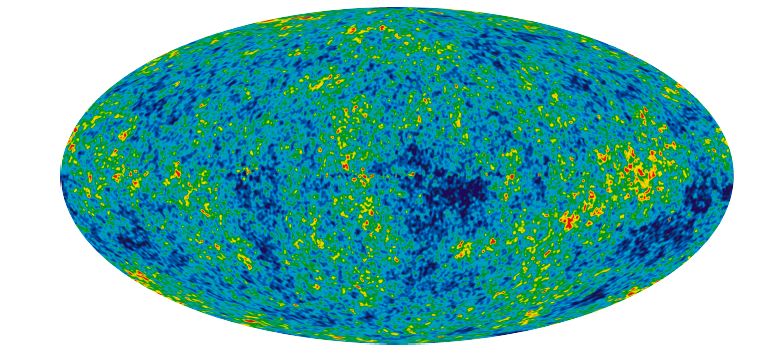
\includegraphics[scale=0.5, angle=0]{cmb.png}
		\caption{Immagine dello spettro della CMB attraverso le misurazioni della sonda spaziale WMAP}
		\label{fig:cmb}
	\end{figure}
\end{center}

Ci muoviamo innanzitutto dal modello cosmologico Einstein-De Sitter, che pone la curvatura dell'universo
e la costante cosmologica $\Lambda$ pari a 0 e prevede uno spazio composto sostanzialmente di materia
oscura fredda (CDM).
In tale cornice definiamo una mappa Lagrangiana $\mathbb{M}: \bm{q} \mapsto \bm{x}(\bm{q}, \tau)$ che connette la posizione
iniziale alla posizione corrente x al tempo di scala $\tau$ $\propto$ $t^{\frac{2}{3}}$.
Inoltre le coordinate x sono coordinate comoventi legate alle coordinate fisiche r dalla relazione
x = r/$a$, dove $a$ rappresenta il fattore cosm
ico di scala, che corrisponde a $\tau$ in un universo
EdS.
Definiamo infine le velocità $\bm{v} = a \dot{\bm{x}}$ e $\bm{w} = \dot{\bm{r}} = H \bm{r} + v$

Per approcciare la dinamica di particelle non collidenti ("polvere"), definiamo una funzione $f(\bm{x}, \bm{p}, t)$ 
che corrisponde alla densità degli stati nello spazio delle fasi. E' possibile quindi utilizzare il Teorema di 
Liouville, che afferma che la densità sopra citata si conserva nell'evoluzione di un sistema conservativo: in
effetti l'ipotesi di assenza di collisioni ci permette di soddisfare ai requisiti del teorema, e quindi 
possiamo porre a zero la derivata totale della funzione densità, ricavando l'equazione di Vlasov.

\begin{equation}
    \label{eqn:vlasov}
    \frac{\partial f}{\partial t} + \dot{\bm{x}} \nabla_{\bm{x}}f + \dot{\bm{p}} \nabla_{\bm{p}}f  = 0
\end{equation}

L'equazione di Vlasov è molto difficile da risolvere analiticamente: adottiamo quindi un approccio 
teorico semplificato, cioè la descizione Newtoniana di fluido: in particolare sposiamo l'ipotesi 
di entropia costante e di assenza di termini di pressione dal momento che trattiamo la CDM come 
una polvere autogravitante e non collidente.

Il set di equazioni adatto all'approccio fluidodinamico è dato da

\begin{equation}
    \label{eqn:continuità}
    \frac{\partial\rho}{\partial t}\biggr|_{\bm{r}} + \nabla_{\bm{r}}(\rho \bm{w}) = 0
\end{equation}

\begin{equation}
    \label{eqn:eulero}
    \frac{\partial\bm{w}}{\partial t}\biggr|_{\bm{r}} + (\bm{w}\cdot\nabla_{\bm{r}})\bm{w} = - \nabla_{\bm{r}} \Phi
\end{equation}

\begin{equation}
    \label{eqn:poisson}
    \laplacian_{\bm{r}}\Phi = 4\pi G \rho
\end{equation}
dove la \ref{eqn:continuità} è l'equazione di continuità che costituisce la conservazione
della massa, la \ref{eqn:eulero} è l'equazione di Eulero e viene dalla conservazione del
momento, mentre la \ref{eqn:poisson} rappresenta l'equazione di Poisson relativa
al potenziale gravitazionale $\Phi$.

Poniamo inoltre $\rho = \rho_b + \delta\rho$, dove $\rho_b$ è la densità media di background
e $\delta\rho$ costituisce una deviazione da tale valore medio. $\Phi = \Phi_b + \phi{'}$ invece
è la somma di un potenziale di background e un potenziale peculiare $\phi{'}$. Grazie a queste due 
apposizioni possiamo separare l'equazione di Poisson, ottenendo un equazione nella sola coordinata
comovente x.
Possiamo riscrivere anche \ref{eqn:eulero} e \ref{eqn:poisson} nelle coordinate x, usando la
relazione

\begin{equation}
    \frac{\partial}{\partial t}\biggr|_{\bm{x}} = \frac{\partial}{\partial t}\biggr|_{\bm{r}} + H(\bm{r} \cdot \nabla_{\bm{r}})
\end{equation}

Si ricava dunque

\begin{equation}
    \label{eqn:continuitax}
    \frac{\partial\rho}{\partial t} + 3H\rho +\frac{1}{2}\nabla_{\bm{x}}(\rho\bm{v}) = 0
\end{equation}

\begin{equation}
    \label{eqn:eulerox}
    \frac{\partial \bm{v}}{\partial t} + H \bm{v} + \frac{1}{a}(\bm{v}\cdot\nabla_{\bm{x}})\bm{v} = -\frac{1}{a}\nabla_{\bm{x}}\phi = 0
\end{equation}

\begin{equation}
    \label{eqn:poissonx}
    \laplacian_{\bm{x}}\phi{'} = 4\pi G \delta\rho
\end{equation}

Le equazioni della fluidodinamica rappresentano in effetti uno sviluppo dell'equazione 
di Vlasov fino al primo ordine. Per spiegare questo passaggio, osserviamo che la densità
di massa e la velocità sono associate rispettivamente al momento di aspettazione di ordine 
zero e di primo ordine della densità nello spazio delle fasi $f(\bm{x}, \bm{p}, t)$.

\begin{equation}
    \label{eqn:rho}
    \rho(\bm{x}, t) = \frac{m}{a^3}\int d^3p f(\bm{x}, \bm{p}, t)
\end{equation}

\begin{equation}
    \label{eqn:vel}
    \bm{v}(\bm{x}, t) = \frac{m}{a^3}\frac{\int d^3p \bm{p}f(\bm{x}, \bm{p}, t)}{\int d^3p f(\bm{x}, \bm{p}, t)}
\end{equation}
Integrando ora l'equazione di Vlasov sul dominio del momento $\bm{p}$, si trova che l'ultimo termine
dell'integrando rappresenta un'integrale di volume della forza $\partial f$/$\partial p$, che tramite
il Teorema di Gauss si può riscrivere come un integrale su una superficie all'infinito, dove la forza
si annulla. Utilizzando poi le definizioni \ref{eqn:rho} e \ref{eqn:vel} si ricava 
\begin{equation}
    \frac{\partial}{\partial t}(a^3 \rho) + \frac{1}{a^2}\nabla_x \int d^3 p \bm{p} f = 0
\end{equation}
maneggiando opportunamente quest'ultima e utilizzando le definzioni fornite in \ref{eqn:rho} e \ref{eqn:vel}
si arriva esattamente all'equazione di continuità \ref{eqn:continuità}.

Se invece si moltiplica l'equazione di Vlasov per $\bm{p}$ per poi integrare di nuovo su tale variabile, 
conviene lavorare sul termine i-esimo e operare un'integrazione per parti sempre sull'ultimo addendo dell'
integrando.

\begin{equation}
    \frac{\partial }{\partial t} \int d^3 p p^i f + \frac{1}{ma^2} \partial^i \int d^3 p p_j p_j f + a^3 \rho \partial^i \phi = 0 
\end{equation}

Manipolando questa espressione e utilizzando l'equazione di continuità, si arriva proprio all'equazione di Eulero
\ref{eqn:eulero}.

Le equazioni della fluidodinamica rappresentano dunque i primi termini dello sviluppo dell'equazione di Vlasov,
e perciò costituiscono una via più facilmente percorribile, offrendo la possibilità di giungere a delle soluzioni
analitiche altrimenti proibitive.


\section{Approssimazione di Zel'dovich}

A questo punto tuttavia conviene operare un ulteriore cambio di variabili sul set di equazioni ottenute \ref{eqn:continuitax},
\ref{eqn:eulerox} e \ref{eqn:poissonx}. Per farlo si definisce meglio il fattore di scala per mezzo di un'ampiezza $a_{*}$ e
un tempo caratteristico $t_{*}$, in modo che $a(t) = (t / t_{*})^{2/3}$. Ricordando inoltre $\rho = \rho_b + \delta\rho$ e 
$\bm{v} = a \dot{\bm{x}}$, facciamo le seguenti sostituzioni

\begin{gather}
    \rho \mapsto \eta = \frac{\rho}{\rho_b} = 1 + \delta \\
    \bm{v} \mapsto \bm{u} = \frac{d\bm{x}}{da} = \frac{d\bm{x}}{dt}\frac{dt}{da} = \frac{\bm{v}}{a\dot{a}} \\
    \phi{'} \mapsto \phi = \frac{3t_{*}^2}{2a_{*}^3}\phi{'}
\end{gather}
Grazie alla mappatura $(\rho, \bm{v}, \phi{'})\mapsto(\eta, \bm{u}, \phi)$, le equazioni del fluido assumono
la nuova forma 

\begin{gather}
    \frac{D\bm{u}}{Da} + \frac{3}{2a}\bm{u} = -\frac{3}{2a}\nabla\phi \\
    \frac{D\eta}{Da} + \eta \nabla \cdot \bm{u} = 0 \\
    \laplacian \phi = \frac{\delta}{a}
\end{gather}
dove la derivata $D/Da$ si dice \textit{derivata convettiva}.
Ora usiamo il fatto che in un universo EdS linearizzato, la soluzione \textit{growing mode} è data complessivamente
da  $\delta \propto t^{\frac{2}{3}}$, $\bm{v} \propto t^{\frac{1}{3}}$ e $\phi = const$. Con questi andamenti, è
evidente che la nuova coordinata di velocità $\bm{u} = \bm{v} / (a\dot{a}) \approx const$, dal momento che sia 
$\bm{v}$ che $a\dot{a} \propto t^{2/3} * t^{-1/3}$ hanno lo stesso andamento $t^{1/3}$.

Ma allora il termine $Du/Da$ nell'equazione di Eulero si può considerare nullo
\begin{equation}
    \label{eqn:zel}
    \frac{Du}{Da} = 0
\end{equation}
ottenendo così

\begin{equation}
    \label{eqn:zelsol}
    \bm{u} = -\nabla\phi
\end{equation}
che è la soluzione linearizzata, valida per piccole deviazioni dalla densità di background, ovvero per $\delta < 1$.
L'approssimazione di Zel'dovich sta nel considerare tale risultato legittimo anche oltre il regime di linearità, ossia 
assumere la validità di \ref{eqn:zel} ovunque.
Si può inoltre osservare che in queste condizioni l'equazione di Poisson gravitazionale risulta disaccoppiata dalle
altre due ed è utile per applicare le condizioni iniziali.
La \ref{eqn:zel} descrive un moto rettilineo uniforme, in cui la particella è soggetta solamente alla propria inerzia
senza perturbazioni gravitazionali esterne. Quindi se la posizione iniziale è descritta dalla coordinata lagrangiana
$\bm{q}$, allora per ogni posizione euleriana $\bm{x}$ del moto varrà che 

\begin{equation}
    \bm{u}(\bm{x}, a) = \bm{u}_0(\bm{q})
\end{equation}
Le traiettorie delle particelle, rettilinee e a velocità costante $u$, sono descritte da

\begin{equation}
    \bm{x}(\bm{q, a}) = \bm{q} + a u_0(\bm{q})
\end{equation}
Ma usando \ref{eqn:zelsol} si ricaverà

\begin{equation}
    \label{eqn:zelmap}
    \bm{x}(\bm{q, a}) = \bm{q} - a \nabla\phi_0
\end{equation}

Alla fine di questi passaggi si è in grado di identificare la mappa $\mathbb{M}$ che collega le coordinate lagrangiane 
iniziali con quelle finali euleriane. 

A questo punto saremmo in grado di risolvere l'equazione di continuità semplicemente come un'equazione a variabili
separabili, trovando quindi la forma di $\eta$. Tuttavia la via più semplice risulta invece dall'impostare la 
conservazione della massa dei singoli elementi fluidi.

\begin{equation}
    \eta(\bm{x}, a)d^3x=\eta_0(\bm{q})d^3q
\end{equation}
da cui

\begin{equation}
    \eta(\bm{x}(\bm{q}, a), a) = (1 + \delta_0(\bm{q}))\det\left(\frac{\partial q}{\partial x}\right) 
\end{equation}
Ma supponendo che nella configurazione iniizale la perturbazione di energia sia nulla $\delta_0 = 0$
e contemporaneamente utilizzando le proprietà del determinante, si potrà scrivere anche

\begin{equation}
    \eta(\bm{x}(\bm{q}, a), a) = \left[\det\left(\frac{\partial x}{\partial q}\right)\right]^{-1}
\end{equation}
E' possibile scrivere la matrice $\partial x$/$\partial q$ in componenti, sapendo che $x_i = q_i - a \frac{\partial\phi_0}{\partial q^i}$, 
e derivando ulteriormente 

\begin{equation}
    \frac{\partial x^i}{\partial q^j} = \delta^i_j - a \frac{\partial^2 \phi_0}{\partial q_i \partial q^j} = 
    \delta^i_j - a D^i_j(q)
\end{equation}
dove si è definito il tensore di deformazione $D^i_j$. Nel sistema di riferimento opportuno tale tensore ha forma
diagonale, con i tre autovalori $\lambda_1(\bm{q})$, $\lambda_2(\bm{q})$ e $\lambda_3(\bm{q})$, dipendenti dalle
coordinate iniziali. Questi governano la deformazione locale della materia lungo i tre assi ortogonali identificati
dagli autovettori. Si può dimostrare che nell'ipotesi in cui il potenziale $phi_0$ sia gaussiano come previsto
dal meccanismo di inflazione, allora nel almeno uno dei tre autovalori del tensore di deformazione è positivo 
nel 92$\%$ dei casi.
Ora, riscrivendo il rapporto di densità $\eta$

\begin{multline}
    \eta(\bm{x}(\bm{q}, a), a) = \left[\det\left(\frac{\partial x}{\partial q}\right)\right]^{-1} = \left[\det\left( \mathbb{I}- a D \right)\right]^{-1} = \\
    = \frac{1}{(1-a\lambda_1(\bm{q}))(1-a\lambda_2(\bm{q}))(1-a\lambda_3(\bm{q}))}
\end{multline}

A questo punto, è evidente che, supponendo che $\lambda_1(\bm{q})$ sia l'autovalore maggiore, allora il tempo 
$\bar{a}=1/\lambda_1(\bm{q})$ rappresenta una criticità, in quanto la quantità $\eta$ diverge e con essa la 
densità. Questo tipo di evento è detto \textit{shell-crossing} o \textit{caustica} ed è rappresenta il 
fenomeno che si registra quando due particelle con diverse coordinate lagrangiane iniziali 
$\bm{q}_1$ e $\bm{q}_2$ confluiscono nella stessa coordinata di campo $\bm{x}$, dando luogo a densità
infinita. 
Tale divergenza è racchiusa nella mancata biunivocità della mappa $\mathbb{M}^{-1}$, dal momento che a 
una sola coordinata euleriana possono corrispondere più coordinate iniziali. A causa della mancanza
di tale biunivocità, la matrice Jacobiana $\partial x/\partial q$ risulta essere mal definita.
Le caustiche delimitano le zone del cosiddetto \textit{multistreaming}, regioni entro le quali non è
più possibile ritracciare le particelle all'indietro, in quanto non sappiamo come si sono comportate
negli eventi di shell-crossing. Le strutture di materia che si formano sono detti \textit{pancakes},
filamenti "quasi" unidimensionali o bidimenzionali, nel senso che la grumosità si sviluppa 
sostanzialmente in una oppure due direzioni. Queste strutture saranno l'opportuna sede la formazione
delle galassie.

Nel regime di single-stream l'approssimazione di Zel'dovich è opportuna, in quanto costitusice 
un modello non accelerato dove le particelle procedono imperturbate lungo una traiettoria rettilinea
 e a velocità costante. Tuttavia a partire dal primo shell-crossing l'approssimazione perde di validità, 
in quanto non prevede effetti di accelerazione gravitazionale esercitata dalle particelle vicine, che 
modificherebbe il cammino della particella in modo sensibile. 

\section{Metodi di ricostruzione}

Come anticipato all'inizio del capitolo, l'alta uniformità della CMB è una prova forte dell'omogeneità 
dell'Universo primordiale. La grumosità della distrubuzione attuale della massa si spiega invece con 
la formazione di strutture filiformi e oblate come i pancakes. Per poter rendere conto di questa transizione,
sono possibili due tipi di atteggiamento: un \textit{forward approach}, che si basa sull'ipotizzare un 
modello iniziale, presumibilmente a densità costante, ed eseguire una simulazione a N corpi sulle basi 
della dinamica Newtoniana, e controllare il grado d'accordo tra l'output della simulazione e la 
distrubuzione attuale delle galassie, per poi accettare o eventualmente rigettare il modello iniziale.
Tale approccio è praticabile solo tramite tecniche numeriche e non permette di formulare analiticamente
il problema a causa del numero troppo elevato di gradi di libertà.

Un modo di ottenere soluzione analitiche invece è seguire un approccio di \textit{reconstruction}, in cui
si tenta di fittare in modo esatto la distribuzione di massa attuale dell'universo e di mappare la velocità 
delle galassie, per poi invertire il problema usando le posizioni attuali come posizioni iniziali e 
cambiando segno alla velocità. 
Tuttavia mentre l'approccio forward, pur con il suo alto coefficiente di difficoltà, si può formulare
in un ben definito problema di Cauchy che garantisca l'unicità delle soluzioni, la reconstruction non
si può formulare allo stesso modo, dato che si è osservato che a causa dello shell-crossing a una 
coordinata euleriana possono corrispondere più posizioni iniziali. Quindi con la ricostruzione si pone 
un problema di condizioni al contorno, per cui la sfida consiste nel trovare un algoritmo che garantisca
unicità.

\begin{center}
	\begin{figure}[H]
		\centering
		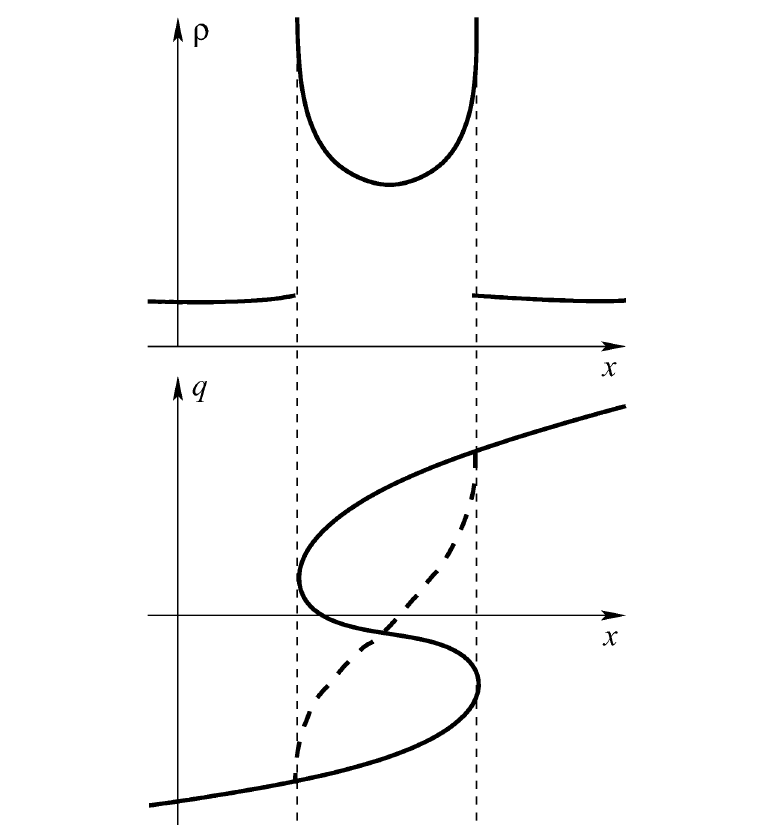
\includegraphics[scale=0.5, angle=0]{rec.png}
        \caption{Esempio di ricostruzione senza unicità. La densità nel grafico superiore potrebbe essere stata generata
        sia dalla mappa lagrangiana in grassetto che da quella tratteggiata. FIgura tratta da \cite{matarrese}}
		\label{fig:rec}
	\end{figure}
\end{center}


Una via percorribile è rappresentata dal problema variazionale come fu formulato da Peebels in \cite{peebles}.
Anzichè risolvere le equazioni del moto, è possibile cercare i punti stazionari della corrispondente
azione di Eulero-Lagrange, scritta nelle coordinate comoventi $\bm{x}$ come

\begin{equation}
    \label{eqn:azione}
    S = \int_0^{t_0} dt \left[\frac{m_i a^2 \dot{\bm{x}}_i^2}{2} - \frac{Gm_i m_j}{a|\bm{x}_i-\bm{x}_j|}+\frac{2}{3}\pi G\rho_ba^2 m_i \bm{x}_i^2\right]
\end{equation}
dove $t_0$ rappresenta il tempo attuale, $\bm{x}_i$ è la traiettoria della i-esima particella e $\rho_b$
è la densità media di background. Se denotiamo come $\mathcal{L}$ l'integrando di \ref{eqn:azione}, allora
è possibile calcolare la variazione di azione e porla uguale a zero per cercare le orbite stazionarie.

\begin{equation}
    \delta S = \int_0^{t_0} dt \left[\frac{\partial \mathcal{L}}{\partial \bm{x}_i}\cdot \delta\bm{x}_i + \frac{\partial\mathcal{L}}{\partial \bm{x}_i}\cdot \delta \dot{\bm{x}}_i\right] = 0 
\end{equation}
Ponendo le opportune condizioni al contorno sarà possibile trovare soluzioni analitiche per $\bm{x}_i$.
In particolare nel suo primo lavoro Peebles considerò solamente i punti di minimo dell'azione: trovò
successivamente che considerando anche i punti di sella si trovava un accordo migliore con i parametri
osservati nel Gruppo Locale.

\begin{center}
	\begin{figure}[H]
		\centering
		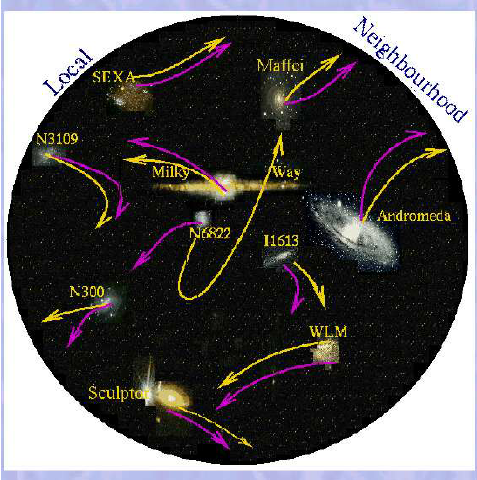
\includegraphics[scale=0.5, angle=0]{peebles.png}
        \caption{Raffigurazione schematica della ricostruzione di Peebles per il Gruppo Locale. Le orbite rosa
        corrispondono alla scelta del minimo dell'azione, mentre quelle gialle indicano la selezione del punto di sella.
        Interessante è il caso della galassia N6822, che offre sia una soluzione in avvicinamento che in allontanamento:
        l'accordo corretto si trova con l'orbita prevista con il punto di sella. Immagine tratta da \cite{mohayaee}.}
		\label{fig:peebles}
	\end{figure}
\end{center}

Tuttavia è impresa ardua ripetere gli stessi risultati su altri set di galassie redshiftate, di cui
sono sconosciute le velocità, necessarie a porre opportune condizioni al contorno. Non è possibile 
quindi scegliere l'orbita corretta tra le molte proposte dall'approccio variazionale, per cui si 
perde l'unicità della soluzione, come accennato in precedenza. 

Oltre all'approccio variazionale appena esposto, un'opzione valida è la ricostruzione POTENT, che si basa
sul rintracciare il campo potenziale della velocità integrando le componenti radiali della velocità.
Questo metodo regge solamente in regime euleriano lineare $|(\rho-\rho_b)/\rho_b|\leq 1$, pertanto non 
recuperano le corrette condizioni iniziali delle regiorni di attuale altà densità, in quanto non lineari:
in altre parole, è un metodo di ricostruzione che non funziona nelle regioni di multistreaming.

Infine il metodo MAK supera sia il problema della non unicità che affligge la ricostruzione di Peebles, 
sia i limiti di validitò dell'algoritmo POTENT, rimanendo valido anche ben oltre il regime lineare euleriano.
Occorre innanzitutto formulare un'equazione di conservazione della massa e prenderla a vincolo

\begin{equation}
    \rho(\bm{x})d\bm{x} = \rho_0(\bm{q})d\bm{q}
\end{equation}
dove $\rho_0(\bm{q})$ è la densità iniziale e a $\rho(\bm{x})$ è la densità alla posizione attuale euleriana.
Manipolando tale equazione di conservazione otterremo 

\begin{equation}
    \label{eqn:masscons}
    \det\left[\frac{\partial q_i}{\partial x_j}\right] = \frac{\rho(\bm{x})}{\rho_0(\bm{q})}
\end{equation}
dove il membro di destra dovrebbe essere noto: conosciamo infatti la posizione della particella
e la densità del campo euleriano, e assumiamo inoltre una densità iniziale costante $\rho_0(\bm{q}) = \rho_0$-
Per risolvere l'equazione, si fa l'ipotesi che la mappa lagrangiana $\mathbb{M}: \bm{q} \mapsto \bm{x}$ si 
possa scrivere come il gradiente di un potenziale convesso $\Phi$.

\begin{equation}
    \bm{x}(\bm{q}, t) = \nabla_q \Phi(\bm{q}, t)
\end{equation}
La convessità del potenziale assicura una relazione biunivoca tra coordinata lagrangiana e coordinata
euleriana, ossia garantisce l'unicità evitando i fenomeni di multistreaming.
Si osserva che nel caso dell'approssimazione di Zel'dovich, con l'equazione \ref{eqn:zelmap} che esplicita la 
mappa lagrangiana è possibile costruire il potenziale $\Phi$, che sarebbe dato da 
$\Phi(\bm{q}, t) = \bm{q}^2/2 -a\phi_0(\bm{q}, t)$.
Tuttavia è evidente che tale potenziale non è convesso ovunque, e proprio per questo l'approssimazione
di Zel'dovich non garantisce unicità, in quanto propone una traiettoria rettilinea secondo cui le particelle 
proseguono dritte nella direzione in cui sono entrate nella zona di shell-crossing, in modo abbastanza irrealistico,
dal momento che la traiettoria di una particella che entra in una zona di alta densità viene presumibilmente modificata in modo 
consistente. 
Sarà invece possibile identificare un potenziale convesso e recuperare quindi l'unicità solamente con una proposta 
alternativa all'approssimazione di Zel'dovich, ossia il modello di adesione, che prevede l'aggiunta di 
termini di interazione gravitazionale.
Se $\Phi$ esiste ed è convesso sarà definita convessa anche la mappa inversa $\Theta(\bm{x}, t)$ tale caustiche
$\bm{q} = \nabla_x \Theta$. La relazione tra $\Phi$ e $\Theta$ è stabilita dalle trasformazioni di
Legendre-Fenchel.

\begin{equation}
    \Theta(\bm{x}) = \max_q \{\bm{q}\cdot\bm{x}-\Phi(\bm{q})\} \qquad \Phi(\bm{q}) = \max_x \{\bm{x}\cdot\bm{q}-\Theta(\bm{x})\}
\end{equation}
A questo punto l'equazione \ref{eqn:masscons} diventa l'equazione di Monge-Ampere.

\begin{equation}
    \det\left[\frac{\partial^2 \Theta (\bm{x}, t)}{\partial x_i \partial x_j}\right] = \frac{\rho(\bm{x})}{\rho_0}
\end{equation}
Solo recentemente si è scoperto che la soluzione a tale equazione è equivalente alla soluzione unica
di un problema di trasporto ottimo, in particolare il problema di trasporto di massa di Monge-Kantorovich,
in cui si cerca quale relazione tra $\bm{q}$ e $\bm{x}$ minimizza la la funzione quadratica di costo 
$c(\bm{q}, \bm{x}) = |\bm{x}-\bm{q}|^2$, o meglio si cerca la minimizzazione del funzionale I.

\begin{equation}
    \label{eqn:mongeampere}
    I = \int_q \rho_0(\bm{q})|\bm{x}-\bm{q}|^2 d\bm{q} = \int_x \rho(\bm{x})|\bm{x}-\bm{q}|^2 d\bm{x} 
\end{equation}
Si trova infatti che per ottenere la condizione $\delta I = 0$, $\bm{q}(\bm{x})$ deve essere il gradiente
di una funzione di $\bm{x}$. I dettagli della trattazione sono reperibili in \cite{mohayaee} e \cite{matarrese}.
Per risolvere l'equazione \ref{eqn:mongeampere} la si discretizza e si risolve il relativo problema di assegnazione 
tramite algoritmi numerici, come quelli presentati in \cite{mohayaee}, che permettano di preservare l'unicità
delle soluzioni.

aaa










\begin{comment}
SCALETTA SEGUENTE
nuova sezione con carrellata su metodi di ricostruzione (citare Mohayaee)
- cos'è la reconstruction
- Peebles
- POTENT
- MAK, particolare attenzione perché prende le origini dalla trattazione fluido
ed è il metodo che fornisce unicità
\end{comment}